\documentclass[a4paper,10pt]{article}
\usepackage{graphicx}
\usepackage{ulem}
\usepackage{anysize}
\usepackage{subfigure}
\marginsize{1cm}{1cm}{1cm}{1cm}
\begin{document}

\begin{flushright}
Michael Ehrlichman\\
\today\\
Memo for BMAD Development\\
\end{flushright}

\begin{center}
\Large
Incorporation of RGS losses into BMAD, following implementation of Touschek losses
\normalsize
\end{center}
\bigskip

Note:  This document has been edited to ``Lab Book'' quality.

\section{Introduction}

Residual Gas Scattering (RGS) occurs when beam particles collide with residual gas molecules.  The energy and angle of the beam particle is changed during the collision.  These changes can result in the particle colliding with the beam chamber downstream of the scattering event.  When the particle is lost to the beam chamber, Bremsstrahlung and neutrons are produced and heat is deposited.  This radiation can pose a hazard to electronics and personell, and the heat can produce leaks in the vacuum chamber.  Because of these hazards, the generation and loss of RGS particles must be examined in detail.

The simulation of RGS losses is similar to that of Touschek losses.  Both are due to single-event scattering processes that change the phase-space coordinate of the colliding particles, resulting in particle loss downstream of the scattering event.  Both processes can be succinctly described by distribution functions that give the rate at which particles with perturbed phase-space coordinated are generated.

Touschek loss simulations have already been implemented in Cornell's beam dynamics code BMAD.
Since the simulation of RGS losses and Touschek losses are similar, the RGS loss simulations will be based upon the 
already developed Touschek loss simulations.

There are two main differences between RGS and Touschek losses.  One difference is the scattering cross-section.  The other difference is that Touschek losses occur only in the horizontal plane, while RGS deflects particles into both the vertical and horizontal plane.

Dealing with the first difference is simple.  Closed formulas for the RGS scattering cross-sections are contained in [\cite{hb}].  These formulas can be integrated numerically to obtain scattering rates that depend on beam parameters, gas parameters, and energy and divergence apertures.

Dealing with the second difference is more involved.  First, the aperture of the accelerator must be determined in the transverse plane for several values of the scattering azimuth.  For example, at $\phi = 0, \pi/4, \pi/2, 3\pi/4, ... 7\pi/4$.  Determining the aperture for various values of $\phi$ is more computationally intensive than determining it in only the horizontal plane, as for Touschek scattering.  However, since the aperture program is parallelized with MPI, the additional computational time is not prohibitive.

\section{Scattering Cross-Sections}

Residual Gas Scattering has two uncorrelated cross-sections.  These are in Section 3.3.1 of [\cite{hb}].  We are interested in elastic and
in inellastic scattering, i.e.  ``Single Coulomb scattering of spin-1/2 particles'' and ``Bremsstrahlung on gas nuclei''.
Coulomb scattering is described by a differential cross-section as a function of zenith.  Bremsstrahlung is described by a 
differential cross-section as a function of fractional energy loss.

\subsection{Angle change due to Coulomb scattering}

Equation 3.3.1.2 from The Handbook gives the differential cross-section for Coulomb scattering as,
\begin{equation}
\frac{d\sigma}{d\theta}\approx 8\pi Z^2 r_e^2 \frac{1}{\left(\theta^2+\theta_{th}^2\right)^2}\left(\frac{m_e c}{\beta p}\right)^2\textrm{,}
\label{diffcross}
\end{equation}
where $\theta_{th}\approx\alpha Z^{1/3}\left(m_e c/p\right)$.  Note that $m_e c/\beta p = \gamma/(\gamma^2-1)$.  Equation (\ref{diffcross}) gives the
differential probability of a particle scattering into a zenith angle $d\theta$.

A scattered particle is lost if $\theta\geq\theta_{min}$, where $\theta_{min}$ is the divergence aperture.  Equation \ref{diffcross} is integrated from $\theta_{min}$ to $\pi$ to obtain the total cross-section for particle loss due to RGS Coulomb scattering. The result is,
\begin{eqnarray}
\sigma_{coul}&=&8\pi Z^2 r_e^2\left(\frac{\gamma}{\gamma^2-1}\right)^2\int_{\theta_{min}}^{\pi}
\frac{1}{\left(\theta^2+\theta_{th}^2\right)^2}\sin\left[\theta\right]d\theta\nonumber\\
&=&8\pi Z^2 r_e^2\left(\frac{\gamma}{\gamma^2-1}\right)^2 \times \left(F\left[\pi\right]-F\left[\theta_{min}\right]\right)\textrm{,}
\label{cross-coul}
\end{eqnarray}
where,
\begin{eqnarray}
F\left[\theta\right]&=&-\frac{1}{8 \theta_{th}^3}\bigg(e^{\theta th}\left(\theta_{th}-1\right)
\left(Ei\left[-\textrm{i}\theta-\theta_{th}\right]+Ei\left[\textrm{i}\theta-\theta_{th}\right]\right)
+e^{-\theta th}\left(\theta_{th}+1\right)
\left(Ei\left[-\textrm{i}\theta+\theta_{th}\right]+Ei\left[\textrm{i}\theta+\theta_{th}\right]\right)\nonumber\\
&&-\frac{4\theta\theta_{th}\sin\left[\theta\right]}{\theta^2+\theta_{th}^2}\bigg)
\textrm{,}
\label{cplx_coul_rgs}
\end{eqnarray}
where $Ei\left[z\right]$ is the exponential integral Ei.  Note that the imaginary part of $Ei$ cancels out
exactly in this expression, guaranteeing a real result.

For storage ring light sources, the equations used for RGS Coulomb scattering are typically much simpler than 
our Eqs. (\ref{cross-coul}) and (\ref{cplx_coul_rgs}).
This is because the beam is always at high energy in a storage ring, in which case $\theta^4 \sim \left(\theta^2+\theta_{min}^2\right)^2$.
This approximation does not apply in an ERL light source, because the beam spans moderate and high energies.

The simulation requires the cross-section for particles scattered into a range $\left[\theta_{min},\theta_{min}+\delta\theta\right]$.
This is because particles with different divergence changes will be lost at different locations.
Unfortunately, the range for Eq. \ref{cross-coul} is $\left[\theta_{min},\pi\right]$.  The required cross-section is obtained 
from $\sigma_{coul}\left[\theta_{min}\right]-\sigma_{coul}\left[\theta_{min}+\delta\theta\right]$.  This formula tells the probability
of a scattering event occuring that gives a particle a divergence in the range $\left[\theta_{min},\theta_{min}+\delta\theta\right]$.

\subsection{Bremsstrahlung on gas nuclei}

Equation (3.3.1.11) from [\cite{hb}] gives the differential cross-section for energy change due to Bremsstrahlung on gas nuclei as,
\begin{equation}
\frac{d\sigma}{du}\approx 4\alpha r_e^2 Z\left(Z+1\right)\frac{4}{3 u}\left(1-u+\frac{3}{4}u^2\right)
\log\left[\frac{184.15}{Z^{1/3}}\right]\textrm{,}
\end{equation}
where $u=k/E$ is the fractional energy loss.  For example, for an $E=5$ GeV particle that loses $k=10$ MeV, $u=0.002$.

The integrated cross-section for a particle to lose an energy between $u_{min}$ and $1$ is,
\begin{equation}
\sigma_{brem}=4\alpha r_e^2 Z(Z+1)\frac{4}{3}\left(-\frac{5}{8}+u_{min}-\frac{3}{8}u_{min}^2-\log\left[u_{min}\right]\right)
\log\left[\frac{184.15}{Z^{1/3}}\right]\textrm{.}
\label{cross-brem}
\end{equation}

The simulations use $\sigma_{brem}\left[u_{min}\right]-\sigma_{brem}\left[u_{min}+\delta u\right]$ to find the probability that
a scattering event occurs that gives a particle an energy change between $u_{min}$ and $u_{min}+\delta u$.

\section{Scattering Rate}

Since Eqs. (\ref{cross-coul}) and (\ref{cross-brem}) do not depend on the phase-space coordinates of the scattering particles or Twiss parameters, a simple derivation is sufficient for determining the rate at which RGS particles are produced.

An electron traveling at a velocity $v$ is incident on a box of dimensions $dx$, $dy$, and $v \Delta t$ containing a density of gas particles $\rho$.  See Fig. \ref{simple-scattering}.
\begin{figure}[h]
  \centering
  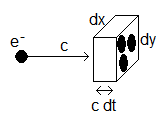
\includegraphics[width=3cm]{simple_scattering.png}\\
  \caption{Simple scattering.}
  \label{simple-scattering}
\end{figure}
The cross-sectional area of each gas particle is $\sigma$.  The box contains $N_\rho=\rho dx dy v \Delta t$ particles, which cover a combined area $A = \sigma\rho dx dy v \Delta t$.  The incident electron has a probability $P=\frac{\sigma\rho dx dy v \Delta t}{dx dy} = \sigma\rho v \Delta t$ of colliding with a gas particle.

A particle traveling through a gas will encounter $\frac{P}{\Delta t}=\sigma\rho v$ collisions per second.  If $N_p$ particles are traveling through the gas as speed $c$, the number of collisions per second will be,
\begin{equation}
\frac{d N_c}{dt dl}=N_p n \sigma c\textrm{.}
\label{basic-rate}
\end{equation}

$N_p$ is set to the number of particles per bunch.  To find the number of scattered particles generated in an element by each crossing bunch, Eq. \ref{basic-rate} is multiplied by $l/c$, where $l$ is the length of the element.

Because Eqs. \ref{cross-coul} and \ref{cross-brem} are uncorrelated, they can be treated as separate processes, each producing a separate distribution of scattered particles.  The rate at which particles are scattered into a range of angle changes by residual gas Coulomb scattering is,
\begin{equation}
\frac{d N_c}{dt}=N_p n l \times\left(\sigma_{coul}\left[\theta_{min}\right]-\sigma_{coul}\left[\theta_{min}+\delta\theta\right]\right)\textrm{,}
\label{coul_rate}
\end{equation}
and the rate at which particles are scattered into a range of energy changed by residual gas Bremsstrahlung scattering is,
\begin{equation}
\frac{d N_c}{dt}=N_p n l \times\left(\sigma_{brem}\left[u_{min}\right]-\sigma_{brem}\left[u_{min}+\delta u\right]\right)\textrm{,}
\label{brem_rate}
\end{equation}

Notice that Eqs. [\ref{coul_rate}] and [\ref{brem_rate}] are functions of only the bunch charge, gas pressure, and the cross-section.  Additionally, 
note that the cross-sections are only functiuons of beam energy and aperture.  The only parameters that change from element-to-element are beam
energy and aperture.  The fact that the formulas do not depend on Twiss parameters means that they do not need to be integrated over the beam
distribution and, as for Touschek losses, and the simulations are greatly simplified.

\section{Determining Aperture}

The divergence and energy apertures for a location in the accelerator are the maximum energy changes and maximum divergence 
change that can be given to a particle at that location without the particle being lost downstream.  The apertures change as you move 
along the accelerator, and so a profile of the apertures needs to be produced.  Typically, it is sufficient re-evaluate the aperture
in $1$ m steps.

For Coulomb scattering with the residual gas, at each slice, the aperture is probed at angles spanning $2\pi$ of azimuth.  The program finds the aperture in $\theta$ at $\phi=0$, then at $\phi=\pi/4$, ..., and finally at $\phi=7\pi/4$.  The aperture in $\theta$ is found using a binary search, changing the divergence of initially on-axis particles.  These results are called the element-by-element divergence aperture of the accelerator.

For Bremsstrahlung due to RGS particles, an aperture for maximum positive energy change and maximum energy change are produced.  These quantities
are also found using a binary search, by changing the energy offset of initially on-axis particles.  These results 
are called the element-by-element energy aperture of the accelerator.

The results for the divergence and energy apertures are each stored in their own data file, which is used by the production 
and tracking simulations.

\section{Production and Tracking}

Since the dimensions of the beam chamber are much larger than the beam envelop, the initial angle and energy defect of the scattered particles can be ignored.  That is, $\delta E/E << u_{min}$ and $\sqrt{\gamma \epsilon} << \theta_{min}$.

\subsection{Coulomb Scattering}

The rate of RGS particles generated by Coulomb scattering at each step along the accelerator is found by numerically integrating Eq.
[\ref{coul_rate}] using the beam energy and aperture at that step and azimuth.  It is assumed that the azimuth of the divergence changes will be 
a flat distribution, and so the rate is divided by the number of azimuths regions.  The azimuth is typically divided into eight regions.

Each test particle is tracked from the element where it is produced to where it is lost.  Because only particles laying outside the divergence
aperture are tracked, all test particles are guaranteed to be lost.  Where the particles are generated and where they are lost is recorded.
Additionally, the trajectories of test particles can also be recorded.

\subsection{Bremsstrahlung on gas nuclei}

The rate of RGS particles generated by Bremsstrahlung scattering is found in a manner similar to that of Coulomb scattering, except that
Eq. [\ref{brem_rate}] is used and instead of evaluating at eight azimuthal apertures, it is evaluated over two energy apertures, the positive 
and negative.

\subsection{Data Analysis}

THE FOLLOWING SECTIONS WILL BE UPDATED WHEN THE CERL 8.0 TOUSCHEK COLLIMATOR DISTRIBUTION IS COMPLETE.

The slice-by-slice generation rate and slice-by-slice loss rate will be generated and recorded.

\section{Results}

Two simulations are produced.  One generates and tracks particles produced by Coulomb scattering, the other by Bremsstrahlung.  The method for constructing the distributions of scattered particles is the same as that for Touschek particles that is described in ``Collimating Touschek particles in an Energy Recovery Linear accelerator,'' Proceedings PAC09.  The simulations results below are from a CERL 7.4 lattice with wiggler collimators but without Touschek collimators.

Shown in Figs. \ref{gen:coul} and \ref{gen:brem} is the current generated per meter due to Coulomb scattering and Bremsstrahlung.  The Coulomb scattering rate is very high at the start of the lattice.  This is due to the $1/\gamma^2$ dependence in Eq. \ref{cross-coul}. $\gamma$ at injection is $20$, and peak $\gamma$ is $10000$.  Since Bremsstrahlung RGS produces only a momentum defect, it produces no scattered particles after the last bend.

\begin{figure}
\subfigure[] % caption for subfigure a
{
    \label{gen:coul}
    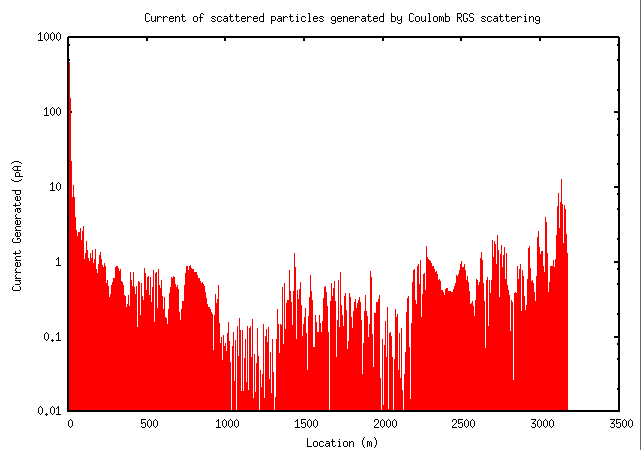
\includegraphics[width=9cm]{gen-coul.png}
}
\subfigure[] % caption for subfigure b
{
    \label{gen:brem}
    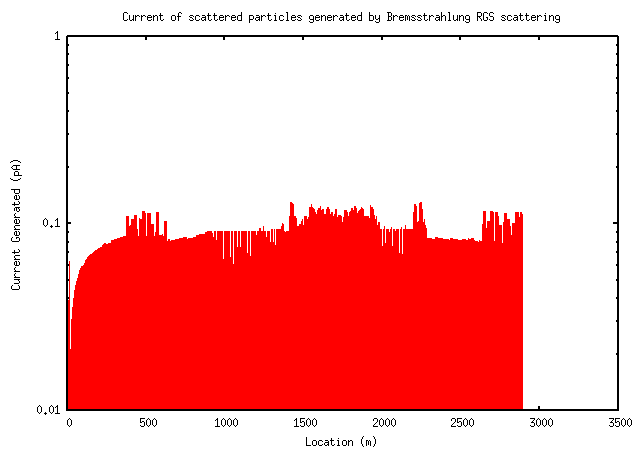
\includegraphics[width=9cm]{gen-brem.png}
}
\caption{Current of lost particles generated per meter due to RGS scattering.}
\label{gen} % caption for the whole figure
\end{figure}

Shown in Figs. \ref{lost:coul} and \ref{lost:brem} is the current lost per meter due to Coulomb scattering and Bremsstrahlung.  Since the Bremsstrahlung process produces only an energy defect, a negligible number of particles are lost in the linacs, where dispersion is zero.

\begin{figure}
\subfigure[] % caption for subfigure a
{
    \label{lost:coul}
    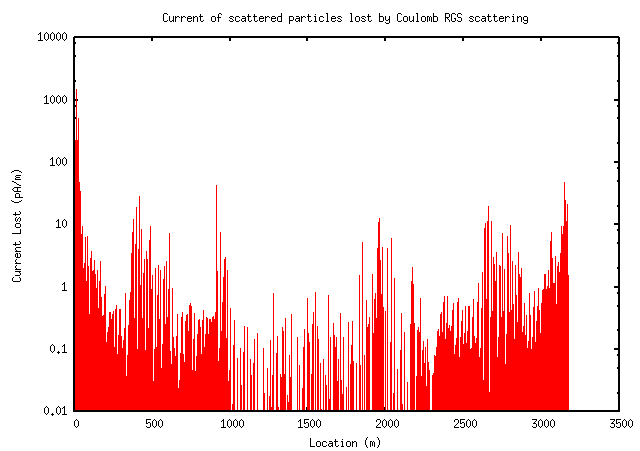
\includegraphics[width=9cm]{lost-coul.png}
}
\subfigure[] % caption for subfigure b
{
    \label{lost:brem}
    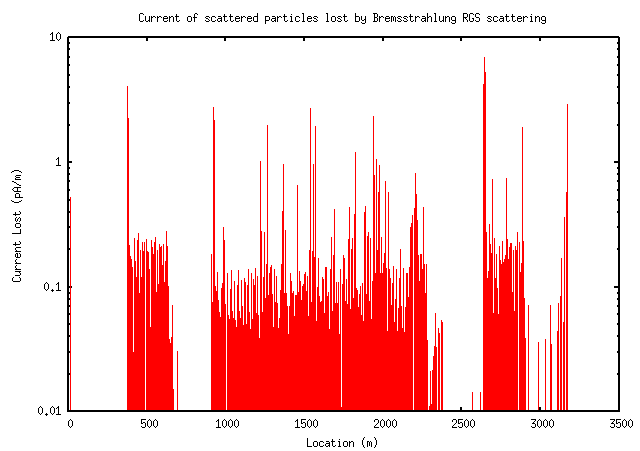
\includegraphics[width=9cm]{lost-brem.png}
}
\caption{Current of particles lost per meter due to RGS scattering.}
\label{gen} % caption for the whole figure
\end{figure}

Shown in Fig. \ref{col:coul} is the distribution of Coulomb RGS particles on the first wiggler collimator.  The histogram grid is $400$ by $400$, giving $3.75 \times 10^{-9}$ m$^2$ per grid point.  Total current is $277.9$ pA.

\begin{figure}[h]
  \centering
  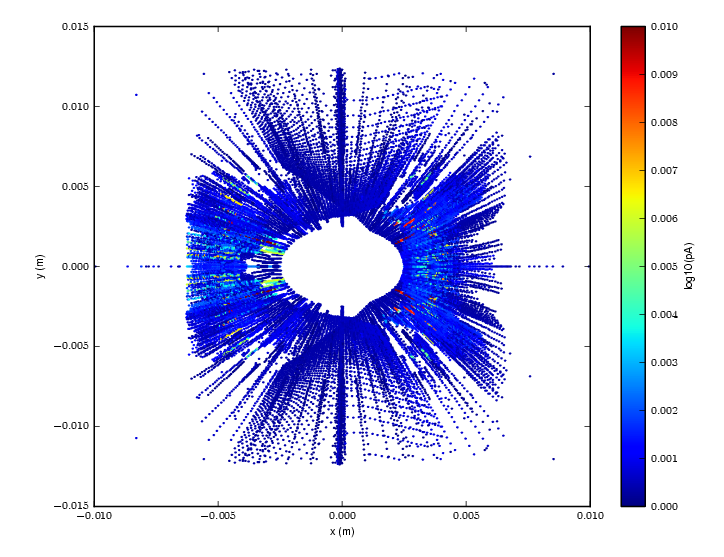
\includegraphics[width=16cm]{coll_dist.png}\\
  \caption{Distribution of Coulomb RGS particles on first wiggler collimator.  Total current in $277.9$ pA. $3.75 \times 10^{-9}$ m$^2$ per grid point.}
  \label{col:coul}
\end{figure}

\section{Conclusion}

Residual Gas Scattering simulations have been implemented in BMAD.  The structure of the simulations is very similar to that of the Touschek simulations.  The RGS simulations have been run on the CERL 7.4 lattice and reasonable results were given.

\begin{thebibliography}{1}
\bibitem{hb} A. Chao, M. Tigner, ``Handbook of Accelerator Physics and Engineering'', (1999)
\end{thebibliography}

\end{document}



